\chapter{Patienten}
Dette kapitel har fokus på patientaspektet, hvor teknologiens påvirkning på patienten vil blive karakteriseret, analyseret og vurderet. 
\section{Metode}
Til analyse af patienten og hvordan teknologien påvirker denne anvendes \autoref{fig:patientaspekter}. Her analyseres sociale forhold, kommunikative forhold, økonomiske forhold, individuelle forhold og etiske forhold, samt sammenspillet mellem disse. I forhold til aktivitetsarmbånd lægges der i denne analyse vægt på sociale forhold, herunder hvordan denne teknologi påvirker patientens arbejds- og uddannelsesliv, familie og livskvalitet, individuelle forhold, herunder hvordan patienten oplever teknologien, kommunikative forhold, herunder hvordan kommunikation fra patient til almen praksis vil forløbe, samt etiske forhold, herunder risiko for misbrug af personlige data. 
%(Nogle af aspekterne kan vægte mere end andre alt efter hvilken teknologi der er tale om, med en aktivitets tracker er det nok mest, (listet i prioriteret rækkefælge) sociale forhold, herunder hvordan det påvirker patientens arbejds/uddannelses liv, familie, fritid og generel livskvalitet. Individuelle forhold, herunder hvordan patienten oplever teknologien, tilfredshed, motivation, tryghed mm. Kommunikative forhold, herunder hvordan der kommunikeres fra f.eks. sygehus til patient og omvendt, fra teknologi til patient og sygehus. Etiske forhold kan måske indgå i og med at patienternes aktivitet måles og bliver opsamlet som data, disse data bliver set af patienten og lægen, måske deler patienten sine resultater over sociale medier, kan disse data misbruges af andre? GPS, placering kan ses. Økonomiske forhold, altså om teknologien giver udgifter for patienten eller påvirker vedkommendes økonomi.).


\begin{figure}[H]
\centering
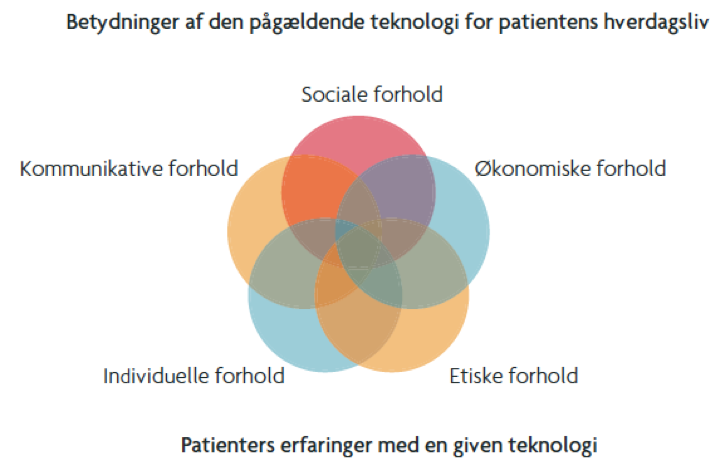
\includegraphics[width=0.8\textwidth]{figures/patientaspekter}
\caption{Patient-aspekter \citep{mtvhaandbog}.}
\label{fig:patientaspekter}
\end{figure}

\noindent
Dette giver anledning til følgende MTV-spørgsmål: 
%(Inklusions og eksklusions kriterier skal muligvis opstilles for at kunne fokusere modellen på den målgruppe som vi vælger at fokusere på)


\subsection{MTV-spørgsmål}
\begin{itemize}
\item Er teknologien brugervenlig og motiverer den patienten til at få en mere aktiv hverdag?
\item Hvordan påvirker teknologien patienternes individuelle og sociale forhold i dagligdagen?
\item Hvor stor en andel af patienter oplever en positiv virkning ved anvendelse af teknologien og hvad spiller en rolle for at teknologien giver et succesfuldt forløb?
\item Hvor meget ansvar har patienten ved anvendelsen af teknologien?
\item Hvad er effekten af at anvende teknologien for patienten og hvad er tidshorisonten på disse effekter? 
\item Er der nogle etiske aspekter ved at monitorere patientens aktivitet, i så fald hvilke dilemmaer opstår heraf?
\item Skal der være bestemte kriterier opfyldt for at patienten kan få en aktivitets tracker?
\end{itemize} 

